\documentclass[11pt]{article}
\usepackage{amsmath}
\usepackage[utf8]{inputenc}
\usepackage{subcaption}%for subfigure
\usepackage{amssymb}%for tilda in math
\usepackage{float}%for forcing position of figs
\usepackage{setspace}
\usepackage{hyperref}
\usepackage{mathptmx}
\usepackage{graphicx}

\title{\large \textbf{Weekly report - 2/13 - 2/20. Imitiation Learning and Policy Optimization}}
\author{Siddharthan Rajasekaran}
\date{}
\usepackage[margin = 1in]{geometry}
 \geometry{
 a4paper,
 top = 15mm,
 }
\linespread{1}
\singlespacing
\begin{document}

\maketitle

\section{Summary}
In this report we will discuss some of the methods to do reinforcement learning (forward control) in high dimensional continuous systems. This is important to us because at every iteration IRL, we have to do solve the forward control to see how good our reward function learned is. This also gives information about out gradient along which we can improve our reward function.

\section{Problems with Value iteration}
Solving the forward problem exactly using value iteration takes $|\mathcal{S}|^2\times |\mathcal{A}|\times |\mathcal{I}|$ computation steps where $\mathcal{S}|$ is the number of states, $|\mathcal{A}|$ is the number of actions and $|\mathcal{I}|$ is the number of minimum number of iterations to converge (which can be proved to be a polynomial in $|\mathcal{S}|$). Clearly, this will not be possible in large or continuous state spaces (which is the case in robotic systems). Hence we go for approximate solutions to the RL problem.

\section{RL for high dimensional/ continuous systems}
The high dimensional problem can be solved using 
\begin{enumerate}
\item Reward Shaping \cite{ng2003shaping}
\item Policy search
\begin{itemize}
\item Cross-Entropy / Evolution Strategy based methods \cite{hansen1996adapting, theodorou2010generalized, kober2009policy, Salimans2017Evolution}
\item Policy Optimization (gradient based) \cite{baxter2001infinite, schulman2015trust}
\end{itemize}
\item Approximate Q learning \cite{van2016deep}
\end{enumerate}

We will discuss Policy search based methods more in detail as they seem promising for our continuous space tasks. We should also explore approximate Q learning based methods in future. Reward shaping however, requires the shaping function to be a difference potential function and has limited capability to scale compared to policy search. 



\subsection{Policy Optimization}
The main motivation behind policy optimization is that it is often hard to define value function or Q function for a specific task. For example, in the task of grasping, one can easily accept a the set of actions (the policy) to be good. However, assigning a value to particular pose during the grasping problem is harder to track \cite{drlnips}. 


 In policy optimization, the way we parameterize the policy $\pi$ using $\theta$. For example, the parameters $\theta$ may be the weights in a huge neural networks that maps states to actions or directly observations to actions. The reinforcement learning objective in the context of policy optimization becomes, 
\begin{align}
  \theta = \arg \max_\theta E[\sum_{t=0}^TR(s_t)|\pi_\theta]
\end{align}
Often stochastic policy class is chosen to smooth out the policy optimization problem in case the underlying reward function is discontinuous. This works better even though we know that we only need a deterministic policy. 

\subsubsection{Cross Entropy Method}

This is a evolution (genetic algorithm) based method. The following shows the algorithm.  

\begin{figure}[H]
  \begin{center}
    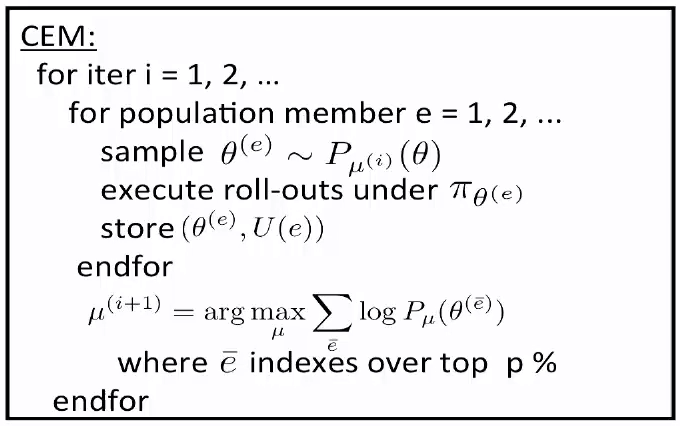
\includegraphics[width=0.7\linewidth]{images/cem.png}
    \caption{Algorithm - Cross Entropy Method}
    \label{fig:cem}
  \end{center}
\end{figure}
 
In the above algorithm we have a parameterized distribution $P_\mu$ for the parameter $\theta$ of the policy. We first sample $n$ parameters from $P_\mu$ that is $\theta^{(e)} \sim P_{\mu^{(i)}}(\theta)$. We execute roll-outs for each of the member in the population and find their cumulative reward $U(e)$. We pick the top $p\%$ individuals with respect to their $U$ of the population and perform a soft-max to update the parameter of our distribution. 

There are several different ways one could update the parameter $\mu$. In \cite{rwr} they perform a reward weighted regression in which the parameter update is given by 

\begin{align}
\mu^{(i+1)} = \arg \max_{\mu} \sum_eq(U(e),P_\mu(\theta^{(e)}))\log{P_\mu(\theta^{(e)}}) 
\end{align}
Here each individual is weighted by a function $q$ of the utility if that individual $U(e)$ and the probability of sampling the parameter $\theta^{(e)}$ from distribution $P_\mu$. In \cite{pi}, instead of picking top $p\%$, you look at all roll-outs and you weigh each roll out by exponentiated utility value $U(e)$ of that roll-out. The update is given by,

\begin{align}
\mu^{(i+1)} = \arg \max_{\mu} \sum_e \exp(\lambda U(e)) \log{P_\mu(\theta^{(e)})}
\end{align}

In \cite{cmaes}, we keep a distribution in a form of a Gaussian  parameterized by mean $\mu$ and covariance $\Sigma$. The update here is given by,
\begin{align}
(\mu^{(i+1)}, \Sigma^{(i+1)}) = \arg \max_{\mu,\Sigma }w(U(\bar{e}))\log{\mathcal{N}(\theta^{(\bar{e}};\mu,\Sigma)}
\end{align}

In \cite{power}, we optimize the expected log probabilities of the roll-outs that we got. The distributions are again assumed to be Gaussian The update here is,
\begin{align}
\mu^{(i+1)} = \mu^{(i)} + \Big(\sum_e(\theta^{(e)}-\mu^{(i)})U(e)\Big)/ \Big( \sum_e U(e) \Big)
\end{align}

This method, called PoWER, has been tested on a rather dynamic task where the robot arm has to swing a ball and drop in a cup it is holding. The link here shows the demonstration of PoWER in action - \url{https://www.youtube.com/watch?v=qtqubguikMk}

The main problem with these methods is that, they work well in case we need to find relatively few parameters. In case we want to learn the parameters of a neural net with hundred thousand parameters, it is difficult to make these methods work. 

Another way to approach this would be to use policy gradient methods. This is where the stochastic policy smooths out a discontinuous reward function. The gaol here can be broadly described as 

\begin{align}
\max_{\theta}U(\theta) = \max_{\theta }\sum_{\tau{}}P(\tau{} ;\theta)R(\tau{})
\end{align}
The gradient is given by 
\begin{align}
\bigtriangledown_\theta U(\theta) = \sum_\tau P(\tau;\theta) \bigtriangledown_\theta \log{P(\tau;\theta)} R(\tau)
\end{align}
Empirically, this is estimated in \cite{gpomdp} as,
\begin{align}
\bigtriangledown_\theta U(\theta) = \frac{1}{m}\sum_{i=1}^m \bigtriangledown_\theta \log{P(\tau;\theta)} R(\tau)
\end{align}
Intuitively, this just moves the parameters in the direction in which the probability of paths with positive R is increased and that of negative R is decreased.  

In a Markovian process, the gradient of the probability $P$ of a path $\tau$ becomes independent of the system dynamics. That is,
\begin{align*}
 \bigtriangledown_\theta \log{P(\tau;\theta)} &=  \bigtriangledown_\theta \log \Big[ \Pi_{t=0}^H P(\cdot)  \pi_{\theta}(\cdot) \Big]\\
 &= \sum_{t=0}^H \bigtriangledown_\theta \log{\pi_\theta(u_t^{(i)}|s_t^{(i)})}
\end{align*}

The bias of the method is proved to be zero and several variance reduction techniques are discussed in \cite{var} for the empirical estimate of the gradient.

In \cite{approx}, they come up with a method that optimizes an approximation to objective function (cumulative reward), a surrogate objective, which makes sure that we monotonically increase the reward while using gradient method. Also, \cite{trpo} guarantees monotonic increase in reward for highly non linear parametric policy such as the ones in neural nets. This allows us to use deep networks for the policy and still apply policy gradient methods. This allows us to effectively combine deep learning and robotics unlike imitation learning.

\section{Conclusion}
The report summarizes some deep learning methods for imitation learning and policy optimization methods. Need to read more on inverse reinforcement learning and form a "Big picture" of how to approach Learning from Demonstration problems. 

\section{Bibliography}

\bibliographystyle{plain}
\bibliography{bibfile} 
%
%\begin{thebibliography}{8}
%\bibitem{cmaes}
%Hansen, Nikolaus, and Andreas Ostermeier. "Adapting arbitrary normal mutation distributions in evolution strategies: The covariance matrix adaptation." Evolutionary Computation, 1996., Proceedings of IEEE International Conference on. IEEE, 1996.
%\bibitem{lstmbirth}
%Hochreiter, Sepp, and Jürgen Schmidhuber. "Long short-term memory." Neural computation 9.8 (1997): 1735-1780.
%\bibitem{rwr}
%Dayan, Peter, and Geoffrey E. Hinton. "Using expectation-maximization for reinforcement learning." Neural Computation 9.2 (1997): 271-278.
%\bibitem{gpomdp}
%Baxter, Jonathan, and Peter L. Bartlett. "Infinite-horizon policy-gradient estimation." Journal of Artificial Intelligence Research 15 (2001): 319-350.
%\bibitem{approx}
%Kakade, Sham, and John Langford. "Approximately optimal approximate reinforcement learning." ICML. Vol. 2. 2002.
%\bibitem{var}
%Greensmith, Evan, Peter L. Bartlett, and Jonathan Baxter. "Variance reduction techniques for gradient estimates in reinforcement learning." Journal of Machine Learning Research 5.Nov (2004): 1471-1530.
%\bibitem{irl}
%Abbeel, Pieter, and Andrew Y. Ng. "Apprenticeship learning via inverse reinforcement learning." Proceedings of the twenty-first international conference on Machine learning. ACM, 2004.
%\bibitem{power}
%Kober, Jens, and Jan R. Peters. "Policy search for motor primitives in robotics." Advances in neural information processing systems. 2009.
%\bibitem{pi}
%Theodorou, Evangelos, Jonas Buchli, and Stefan Schaal. "A generalized path integral control approach to reinforcement learning." Journal of Machine Learning Research 11.Nov (2010): 3137-3181.
%\bibitem{dagger}
%Ross, Stéphane, Geoffrey J. Gordon, and Drew Bagnell. "A Reduction of Imitation Learning and Structured Prediction to No-Regret Online Learning." AISTATS. Vol. 1. No. 2. 2011.
%\bibitem{trpo}
%Schulman, John, et al. "Trust Region Policy Optimization." ICML. 2015.
%\bibitem{nvidia}
%Bojarski, Mariusz, et al. "End to end learning for self-driving cars." arXiv preprint arXiv:1604.07316 (2016).
%\bibitem{lstm}
%Rahmatizadeh, Rouhollah, et al. "Learning real manipulation tasks from virtual demonstrations using LSTM." arXiv preprint arXiv:1603.03833 (2016).
%\bibitem{drlnips}
%Shulman, Abbeel. Deep Reinforcement Learning Through Policy Optimization. NIPS 2016. https://goo.gl/TACjs6
%\bibitem{walking}
%\url{https://www.youtube.com/watch?v=kl_G95uKTHw&t=1305s}
%\end{thebibliography}
\end{document}

